\documentclass[a4paper,10pt]{article}
 
\usepackage[T1]{fontenc}
\usepackage[utf8]{inputenc}
\usepackage{graphicx}
\usepackage{xcolor, colortbl}
\usepackage{caption}
\usepackage{listings}
\usepackage{wrapfig} 
\usepackage{tabu} % For coloring single row of table
\usepackage{scrextend}

\renewcommand\familydefault{\sfdefault} 
\usepackage{tgheros}
\usepackage[defaultmono]{droidmono}

\usepackage{amsmath,amssymb,amsthm,textcomp}
\usepackage{enumerate}
\usepackage{multicol}
\usepackage{tikz}

\usepackage{geometry}
\usepackage{trace}
\usepackage{tcolorbox}
\usepackage{tabularx}
\usepackage{accsupp}% http://ctan.org/pkg/accsupp


\tcbuselibrary{listings,skins} % For lstlisting

\geometry{total={210mm,297mm},
left=25mm,right=25mm,%
bindingoffset=0mm, top=20mm,bottom=20mm}


% For coloring single row in table
\def\zapcolorreset{\let\reset@color\relax\ignorespaces}
\def\colorrows#1{\noalign{\aftergroup\zapcolorreset#1}\ignorespaces}

\newcommand{\linia}{\rule{\linewidth}{0.5pt}}
\newcommand{\ano}{\text{0}}

% custom theorems if needed
\newtheoremstyle{mytheor}
    {1ex}{1ex}{\normalfont}{0pt}{\scshape}{.}{1ex}
    {{\thmname{#1 }}{\thmnumber{#2}}{\thmnote{ (#3)}}}

\theoremstyle{mytheor}
\newtheorem{defi}{Definition}

% my own titles
\makeatletter
\renewcommand{\maketitle}{
\begin{center}
\vspace{2ex}
{\huge \textsc{\@title}}
\vspace{1ex}
\\
Department of Electronics and Communication Engineering \\
Indian Institute of Technology, Roorkee
\linia\\
ECN 104 \hfill Digital Logic Design
\vspace{4ex}
\end{center}
}
\makeatother
%%%

% custom footers and headers
\usepackage{fancyhdr}
\pagestyle{fancy}
\lhead{}
\chead{}
\rhead{}
\lfoot{Assignment \ano\ - Template}
\cfoot{}
\rfoot{Page \thepage}
\renewcommand{\headrulewidth}{0pt}
\renewcommand{\footrulewidth}{0pt}
%

\definecolor{vgreen}{RGB}{104,180,104}
\definecolor{vblue}{RGB}{49,49,255}
\definecolor{vorange}{RGB}{255,143,102}

\makeatletter
\newcommand*\@lbracket{[}
\newcommand*\@rbracket{]}
\newcommand*\@colon{:}
\newcommand*\colorIndex{%
    \edef\@temp{\the\lst@token}%
    \ifx\@temp\@lbracket \color{black}%
    \else\ifx\@temp\@rbracket \color{black}%
    \else\ifx\@temp\@colon \color{black}%
    \else \color{vorange}%
    \fi\fi\fi
}
\makeatother

\definecolor{codebg}{RGB}{250,250,240} 
\definecolor{greatblue}{RGB}{91,155,215} 

% Set up caption and labels for lstlistings
\DeclareCaptionFont{white}{\color{white}}
\DeclareCaptionFormat{listing}{\colorbox{greatblue}{\parbox{\textwidth}{\hspace{1cm}#1#2#3}}}
\captionsetup[lstlisting]{format=listing,labelfont=white,textfont=white}

\renewcommand{\thelstnumber}{% Line number printing mechanism
  \protect\BeginAccSupp{ActualText={}}\arabic{lstnumber}\protect\EndAccSupp{}%
}

\def\backtick{\char18} 
\lstdefinestyle{verilog-style}
{
    %columns=fullflexible, 
    language=Verilog,
    basicstyle=\small\ttfamily,
    keywordstyle=\color{vblue},
    identifierstyle=\color{black},
    commentstyle=\color{vgreen},
    numbers=left, 
    numberstyle=\color{gray},  
    numbersep=10pt,
    moredelim=*[s][\colorIndex]{[}{]},
    literate=*{:}{:}1, 
    backgroundcolor=\color{codebg},
    framexrightmargin=0.09cm, 
    framexleftmargin=-0.09cm,
    frame=trbl,
    upquote=true, 
    framerule=0pt,
    keepspaces=true
}

\newcommand{
  \insertverilog}[3]{
  \lstinputlisting[label=#2, caption=#3, style={verilog-style}]{#1}
}

% Command for problem
\newcounter{problemNumber}
\setcounter{problemNumber}{1}
\newcommand {
  \insertProblem}[1]{
  \vspace{0.5cm}
  \hrule
  \vspace{0.3cm}

  {\color{greatblue}\textbf{\large{Problem \theproblemNumber}}}
  \vspace{2pt}\\#1

  \addtocounter{problemNumber}{1}
  \vspace{0.2cm}
  \hrule  
  \vspace{0.5cm}
}


%%%----------%%%----------%%%----------%%%----------%%%
% Command for creating a resource box
\newcommand{\resourcebox}[2]{
  \fbox{%
    \parbox{0.5\textwidth}{%
      \text{#1}
    }%
  } 
}


%%%----------%%%----------%%%----------%%%----------%%%

\makeatletter
\def\lst@outputspace{{\ifx\lst@bkgcolor\empty\color{white}\else\lst@bkgcolor\fi\lst@visiblespace}}
\makeatother


%%%----------%%%----------%%%----------%%%----------%%%
\begin{document}

\title{Assignment \ano \\ Template}

\maketitle

\section*{Section}
Lorem ipsum dolor sit amet, consectetuer adipiscing elit.  Donec hendrerit tempor tellus.  Donec pretium posuere tellus.  Proin quam nisl, tincidunt et, mattis eget, convallis nec, purus.  Cum sociis natoque penatibus et magnis dis parturient montes, nascetur ridiculus mus.  Nulla posuere.  Donec vitae dolor.  Nullam tristique diam non turpis.  Cras placerat accumsan nulla.  Nullam rutrum.  Nam vestibulum accumsan nisl.

Nullam eu ante vel est convallis dignissim.  Fusce suscipit, wisi nec facilisis facilisis, est dui fermentum leo, quis tempor ligula erat quis odio.  Nunc porta vulputate tellus.  Nunc rutrum turpis sed pede.  Sed bibendum.  Aliquam posuere.  Nunc aliquet, augue nec adipiscing interdum, lacus tellus malesuada massa, quis varius mi purus non odio.  Pellentesque condimentum, magna ut suscipit hendrerit, ipsum augue ornare nulla, non luctus diam neque sit amet urna.  Curabitur vulputate vestibulum lorem.  Fusce sagittis, libero non molestie mollis, magna orci ultrices dolor, at vulputate neque nulla lacinia eros.  Sed id ligula quis est convallis tempor.  Curabitur lacinia pulvinar nibh.  Nam a sapien.

\subsection*{Sub Section} 
Pellentesque dapibus suscipit ligula.  Donec posuere augue in quam.  Etiam vel tortor sodales tellus ultricies commodo.  Suspendisse potenti.  Aenean in sem ac leo mollis blandit.  Donec neque quam, dignissim in, mollis nec, sagittis eu, wisi.  Phasellus lacus.  Etiam laoreet quam sed arcu.  Phasellus at dui in ligula mollis ultricies.  Integer placerat tristique nisl.  Praesent augue.  Fusce commodo.  Vestibulum convallis, lorem a tempus semper, dui dui euismod elit, vitae placerat urna tortor vitae lacus.  Nullam libero mauris, consequat quis, varius et, dictum id, arcu.  Mauris mollis tincidunt felis.  Aliquam feugiat tellus ut neque.  Nulla facilisis, risus a rhoncus fermentum, tellus tellus lacinia purus, et dictum nunc justo sit amet elit.

\subsection*{Sub Section } 
Lorem ipsum dolor sit amet, consectetuer adipiscing elit.  Donec hendrerit tempor tellus.  Donec pretium posuere tellus.  Proin quam nisl, tincidunt et, mattis eget, convallis nec, purus.  Cum sociis natoque penatibus et magnis dis parturient montes, nascetur ridiculus mus.  Nulla posuere.  Donec vitae dolor.  Nullam tristique diam non turpis.  Cras placerat accumsan nulla.  Nullam rutrum.  Nam vestibulum accumsan nisl.

\begin{figure}[h] \centering 
  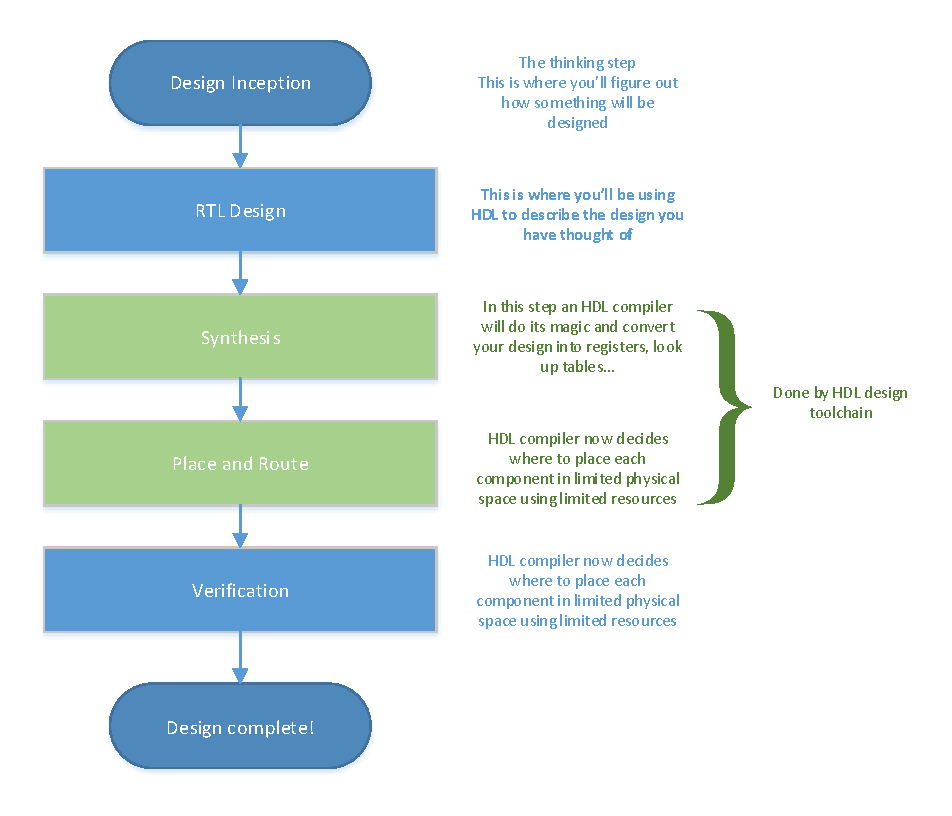
\includegraphics[width=\linewidth]{./resources/hdl_design_flow.pdf}
  \caption{Basic design flow of a design from its inception to implementation.}
  \label{Fig:bst_sample_names}
\end{figure}

\subsubsection*{Sub Sub Section}
Nullam eu ante vel est convallis dignissim.  Fusce suscipit, wisi nec facilisis facilisis, est dui fermentum leo, quis tempor ligula erat quis odio.  Nunc porta vulputate tellus.  Nunc rutrum turpis sed pede.  Sed bibendum.  Aliquam posuere.  Nunc aliquet, augue nec adipiscing interdum, lacus tellus malesuada massa, quis varius mi purus non odio. 
\subsubsection*{Sub Sub Section}
Pellentesque dapibus suscipit ligula.  Donec posuere augue in quam.  Etiam vel tortor sodales tellus ultricies commodo.  Suspendisse potenti.  Aenean in sem ac leo mollis blandit.  Donec neque quam, dignissim in, mollis nec, sagittis eu, wisi.  Phasellus lacus.  Etiam laoreet quam sed arcu.  Phasellus at dui in ligula mollis ultricies.

\pagebreak
\insertProblem{
  Lorem ipsum dolor sit amet, consectetuer adipiscing elit.  Donec hendrerit tempor tellus.  Donec pretium posuere tellus.  Proin quam nisl, tincidunt et, mattis eget, convallis nec, purus.
}

\begin{table}[h]
  \begin{center}
    \label{Table:operators-table}
    \caption{List of common operators used in Verilog}
    \renewcommand{\arraystretch}{1.1}
    \begin{tabularx}{.8\textwidth}{|X|X|X|} 
      \hline
      \rowcolor{greatblue}
      \color{white}  Operator & \color{white}Description & \color{white}Functional Group \\
      %  \colorrows{\color{black}} 
      \hline
      \text{[]} & bit select or part select &  \\
      
      \hline
      \text{()} & parenthesis &  \\
      
      \hline
      \text{!} & negation &  logical\\
      \text{\textasciitilde} & negation &  bit\-wise\\
      \text{\&} & reduction AND & reduction \\
      \text{\textbar} & reduction OR & reduction \\
      \text{\textasciitilde\&} & reduction NAND & reduction \\
      \text{\textasciitilde\textbar} & reduction NOR & reduction \\
      $^\wedge$ & reduction XOR & reduction \\
      \textasciitilde$^\wedge$ or $^\wedge$\textasciitilde & reduction XNOR & reduction \\
      \hline
      $+$ & Unary Plus (plus sign) & airthmetic \\
      $-$ & Unary minus (minus sign) & \\
      \hline
      $*$ & multiply & airthmetic \\
      $/$ & divide &  \\
      \% & modulus &  \\
      \hline
      \text{\&} & bitwise AND & bitwise \\
      \text{\textbar} & bitwise OR & \\
      \text{\textasciitilde} & bitwise XOR & \\
      \hline
    \end{tabularx}
  \end{center}
\end{table}

\section*{References}
\begin{itemize}
  \small 
\item Nullam eu ante vel est convallis dignissim.  
\item Aenean in sem ac leo mollis blandit.  
\end{itemize}

\end{document}

